\chapter{Experimental part: Exploratory data analysis}
\label{chap:dataexplore}
In this chapter, we will explore the data we have, create several new features from existing ones, visualize and discover the relationships between them. Most of the figures and tables for this chapter you can find in \nameref{appendix}.\\

Here we often refer to a \textit{meta name} field in the dataset. It may takes five values: \textit{name}, \textit{startDate}, \textit{location}, \textit{description} and \textit{noEvent}. Also we use the term \textit{event component} which is applied to all meta names excluding \textit{noEvent}.


\section{Feature engineering}
Before we start exploring the data, we would like to extract several new features. We will work on the following types of features: 

\begin{itemize}
\item \textit{Textual features} related to an original text of the event components.
\item \textit{Spatial features} related to X and Y coordinates of the web element on the page. X and Y are coordinates of a visual block on the real rendered page. 
\end{itemize}

In section \nameref{sec:css} we already extracted several \textit{Visual features} from the CSS properties. We divided into three parts a value of color, the font family and properties measured the pixels. 

\subsection{Textual features}

An original textual feature is a text contained in a web element. For the event name, location and start date, it's a quite short string. For a description is much longer text. That's why the first extracted feature is a \textit{length of the text}. On the figure \ref{fig:distrTextByMeta} you distribution of the text length differs among meta names. \\

After we had extracted the text length, we noticed that the date and location meta names usually contain more digits than name and description. So we derived also the number of digits in a text. See figure \ref{fig:distrDigitsByMeta}.\\

By analogy, we also extracted the number of uppercase letter, white spaces, digit proportion and the number of punctuation marks. See the rest of the figures in \nameref{appendix}.

\begin{figure}[h]
\begin{subfigure}{.5\textwidth}
  \centering
  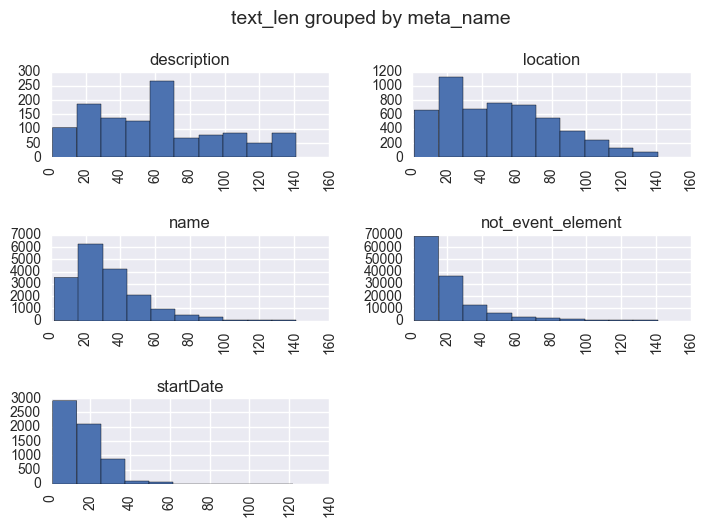
\includegraphics[width=1\textwidth]{figures07/distrTextByMeta}
  \caption{Histogram}
\end{subfigure}
\begin{subfigure}{.5\textwidth}
  \centering
  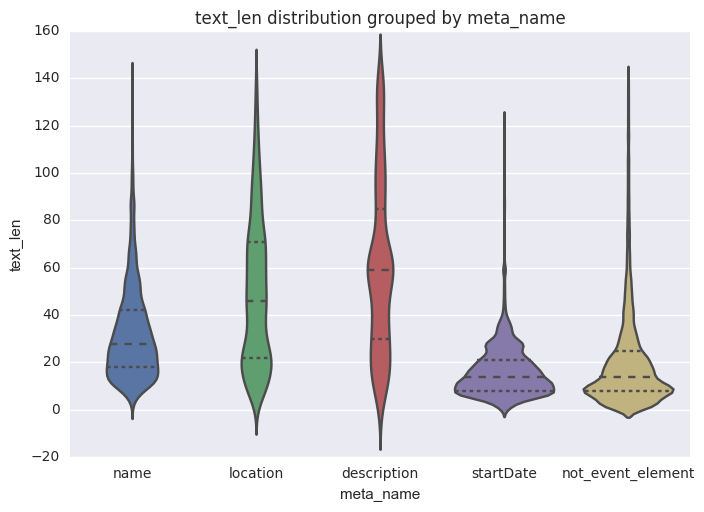
\includegraphics[width=1\textwidth]{figures07/distrTextByMeta_violin}
  \caption{Violin plot}
\end{subfigure}
\caption{Distribution of the text length by meta name}
\label{fig:distrTextByMeta}
\end{figure}


\begin{figure}[h]
\begin{subfigure}{.5\textwidth}
  \centering
  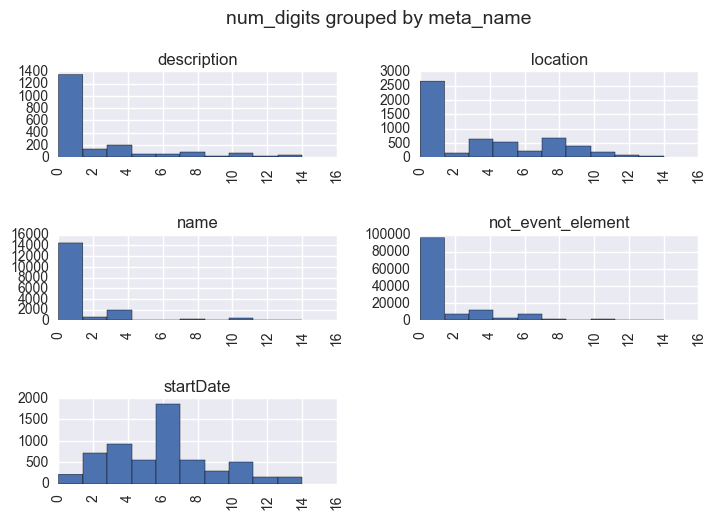
\includegraphics[width=1\textwidth]{figures07/distrDigitsByMeta}
  \caption{Histogram}
\end{subfigure}
\begin{subfigure}{.5\textwidth}
  \centering
  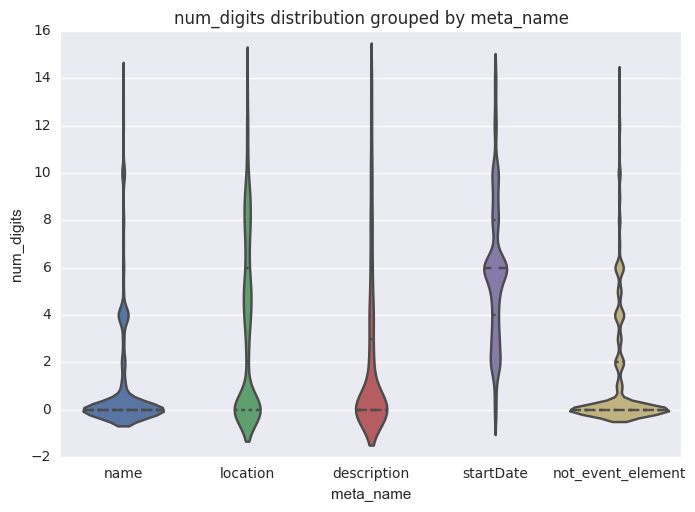
\includegraphics[width=1\textwidth]{figures07/distrDigitsByMeta_violin}
  \caption{Violin plot}
\end{subfigure}
\caption{Distribution of the digits number by meta name}
\label{fig:distrDigitsByMeta}
\end{figure}

Therefore we created six additional features from one textual field: text length, the number of punctuation marks, the number of digits, digits share, the number of upper case letters, the number of white spaces. You can see that visually they distinguish meta names well. The difference in basic statistics you can find in table \ref{table:textualDistr}. \\

When we build different classification models in the next chapter, we will also calculate a \textit{tf-idf weighting matrix} in order to reflect the importance of every word in a text.

\subsection{Spatial features}

Here we will work on two original coordinates X and Y of visual blocks. The visual block is a rectangle on a webpage where the web element is located. Also, we will use two other related features: block width and block height. The precise meaning of X, Y features as follows: X pixels means horizontal position on a page from the left side, and Y pixels means vertical position on a page from the top side. That means that X and Y are coordinates of the left upper corner of the corresponding visual block. An example of X-Y scatter plot you can see on figure \ref{fig:startDateXY}. The axes on inverted such it looks the same as on a webpage.\\

The first feature we created, is an ultimate X and Y which are centers of the visual block rather than left the upper corner. Our guess was that these two features better represent the location on the page. We visualized these two coordinates, and it appears that there is no clear pattern here, rather the elements can appear almost anywhere on a page with only small deviation in means. See the figure \ref{fig:xyLocNameDate}.\\

\begin{figure}[h]
\begin{subfigure}{.5\textwidth}
  \centering
    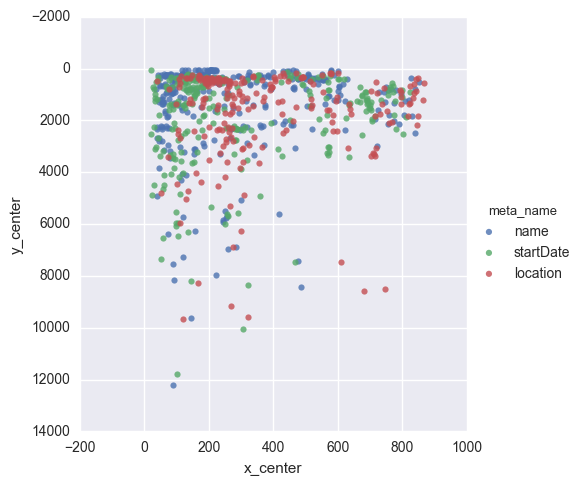
\includegraphics[width=1\textwidth]{figures07/xyLocNameDate}
    \caption{Centers of block coordinates for different meta names which appear on the same page}
    \label{fig:xyLocNameDate}
\end{subfigure}
\begin{subfigure}{.5\textwidth}
  \centering
    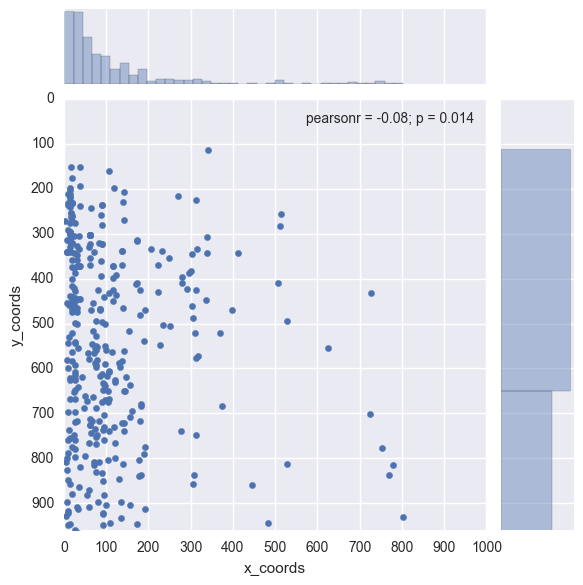
\includegraphics[width=.85\textwidth]{figures07/startDateXY}
    \caption{Original X and Y for an event start date}
    \label{fig:startDateXY}
\end{subfigure}
\caption{The distribution of X and Y coordinates}
\end{figure}


Then we applied K-means clustering algorithm to assign the cluster label for every row. The idea here was to attempt the visual block on a page where every component might appear. We learned the model for sub-datasets for every meta name. Unfortunately, this experiment wasn't successful, because it seems that centered X and Y don't have a clustering structure. There is some difference in basic statistics of X and Y for different meta names, but the standard deviation is so high that it can't be considered as a significant result, see the table \ref{table:spatialDistr}.


We can make several conclusions on the spatial features:
\begin{itemize}
    \item Visually X and Y coordinates badly separate the meta names.
    \item The average of X coordinate differs for all meta names, but the standard deviation is very high. Y coordinates are more or less the same for all meta names except the description, usually, it's located lower than other components.
    \item Both, the visualization and summary statistics may be interpreted as follows: generally, the name is located higher, the start date is more on the left side, the start date is usually more left than the location, and description is below. From page to page the design is different, and that's why there is no clear picture on component locations. Since in our work we build one-vs-all classifiers, we won't use the relative positions of the event components.     
\end{itemize}

% \begin{figure}[h]
% \begin{center}
% 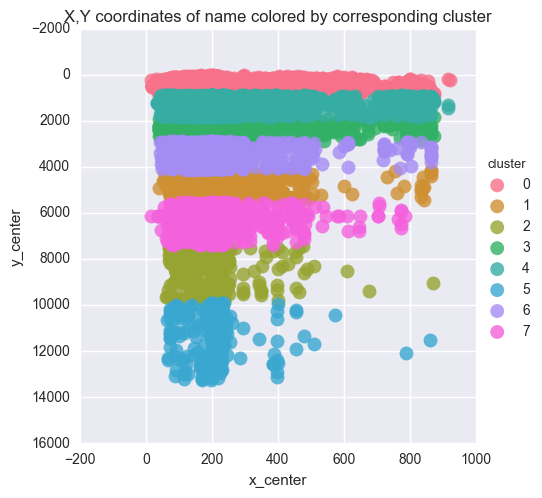
\includegraphics[width=.6\textwidth]{figures07/nameXYCluster8}
% \caption{Unsuccessful clustering of X,Y center of the blocks for event name, K = 8}
% \label{fig:nameXYCluster8}
% \end{center}
% \end{figure}    

\section{The final dataset}
The final dataset after the cleaning and feature engineering is a table of 168K rows and 32 columns. Let's look at its main properties: 

\begin{itemize}
    \item The list of features in the dataset can be seen in table \ref{table:featurelist}.
    \item Every row in a dataset associated with one of the following meta names for every parsed URL: event name, event date, event location, event description or random element on the page. The row contains URL, meta name and all web features we collected: textual, spatial, visual and DOM-related.
    \item It's cleaned of outliers, frequent domains, multi-events pages, and inconsistency. 
    \item It contains 33K unique URLs and  4000 domain names. 
    \item There are in average 45 URLs per one domain name. 
    \item We have 137K rows related to random elements on the webpage, 18K for an event's name, 6K for a start date, 6K for location, and 2K for description. In sum, 32K rows containing features of event components. 
    \item There are in average 1.8 event components out of 4 on a webpage. 
    \item There are the most popular combinations of event components fro one URL. 
    \begin{itemize}
        \item \textit{name} 8335
        \item \textit{location, name} 2863 
        \item \textit{name, startDate} 2522 
        \item \textit{location, name, startDate} 1735
    \end{itemize}
    Top 10 list of combinations you may find in table \ref{table:top10comb}.
    \item We have 30 numeric features and 4 textual. Additionaly, we will include \textit{idf-idf} matrix later.
    \item We replaced outliers of numerical features with the NaN. We fill the missing values with the corresponding average values.
\end{itemize}


\begin{table}[h]
\begin{center}
{\renewcommand{\arraystretch}{1.2}
\begin{tabular}{| p{6cm} | p{6cm} |}
\hline
\textbf{DOM}   &   \textbf{CSS (Visual)}\\
\hline
URL of the page    &    Color (three chanells)\\
Meta name (name, startDate, description, location, no\_event)    &    Text alignment (center, left, right, etc)    \\
Text of the web element    &    Property of the block view    \\
HTML tag    &    The level font weight    \\
Number of siblings in a DOM tree    &    Padding    \\
Number of childs in a DOM tree    &    Font family (Verdana, Arial, etc)    \\
    &    Font size \\
    &    The language of the page \\
\hline
\textbf{Spatial}   &   \textbf{Textual}  \\
\hline
X and Y coordinate on the rendered picture    &    Length of the text inside the block    \\
X and Y coordinate of the center of a visual block    &    Number of punctuation marks in text    \\
Visual block height     &    Number of digits in text    \\
Visual block width        &    Number of digits/text length    \\
Height in a browser     &    Number of upper case letters    \\
Width in a browser     &    Number of whitespaces    \\

     &    \textit{+ tf-idf matrix}    \\
\hline
\end{tabular}}
\caption{The final list of features}
\label{table:featurelist}
\end{center}
\end{table}    

\begin{table}
\begin{center}
{\renewcommand{\arraystretch}{1.5}
\begin{tabular}{| p{8cm} | p{2cm}|}
\hline
\textbf{Combination}    &    \textbf{Count}\\
\hline
['name']    &    8335\\
\hline
['location', 'name']    &    2863\\
\hline
['name', 'startDate']    &    2522\\
\hline
['location', 'name', 'startDate']    &    1735\\
\hline
['description', 'name']    &    730\\
\hline
['description', 'name', 'startDate']    &    548\\
\hline
['description', 'location', 'name']    &    485\\
\hline
['description', 'location', 'name', 'startDate']    &    293\\
\hline
['name', 'startDate', 'startDate']    &    246\\
\hline
['location', 'name', 'startDate', 'startDate']    &    125\\
\hline
\end{tabular}}
\caption{Top 10 combinations of event component for every URL}
\label{table:top10comb}
\end{center}
\end{table}    

\section{Analysis of features}
Let's briefly mention other valuable features which separate the meta name well enough. We will present the visualization with the grouping by the meta name and some summary tables.

On the figure \ref{fig:boxUpperByMeta} we can see that the number of uppercase letters is the highest for location meta name and the lowest for a start date.\\

The figure \ref{fig:distrFontSizeByMeta} shows that the distribution of a font size has a very different shape for different meta names. For description, it is more or less normal, for the name and start date it is right-skewed distribution, and for a random element it is almost stable which says that the random elements of the page in average has the same font size.\\   

Basic statistics for the different numerical features for all meta names you can see on table \ref{table:sumstatnum}.\\

On the figure \ref{fig:distrTagByMeta} you will notice that the tag usage is different for different meta names. We encoded the tag name by the number from 0 to 35.  \\

\begin{figure}[h]
\begin{subfigure}{.5\textwidth}
  \centering
  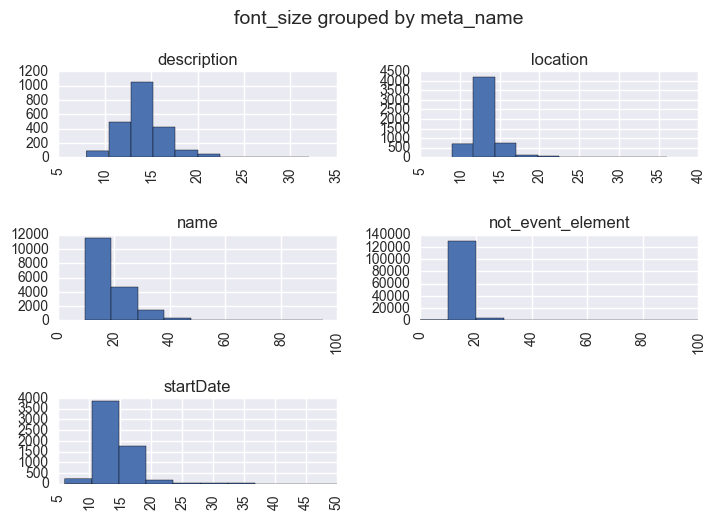
\includegraphics[width=1\textwidth]{figures07/distrFontSizeByMeta}
  \caption{The font size by meta names}
  \label{fig:distrFontSizeByMeta}
\end{subfigure}
\begin{subfigure}{.5\textwidth}
  \centering
    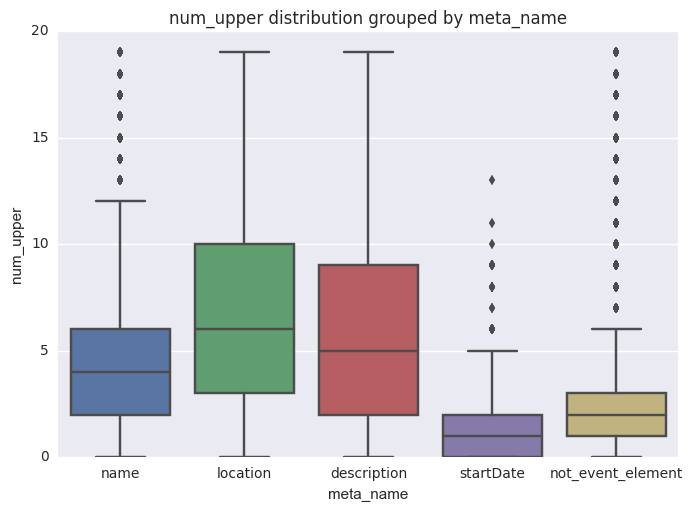
\includegraphics[width=1\textwidth]{figures07/boxUpperByMeta}
    \caption{The number of uppercase letters by meta names}
    \label{fig:boxUpperByMeta}
\end{subfigure}
\caption{Distribution of digits number by meta name}
\end{figure}

\begin{figure}[h]
\begin{subfigure}{.5\textwidth}
  \centering
  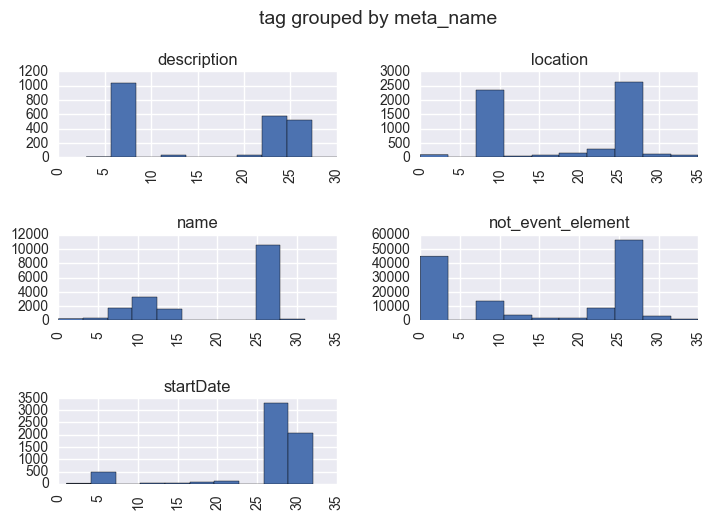
\includegraphics[width=1\textwidth]{figures07/distrTagByMeta}
  \caption{Distribution of HTML tag value by meta names}
  \label{fig:distrTagByMeta}
\end{subfigure}
\begin{subfigure}{.5\textwidth}
  \centering
    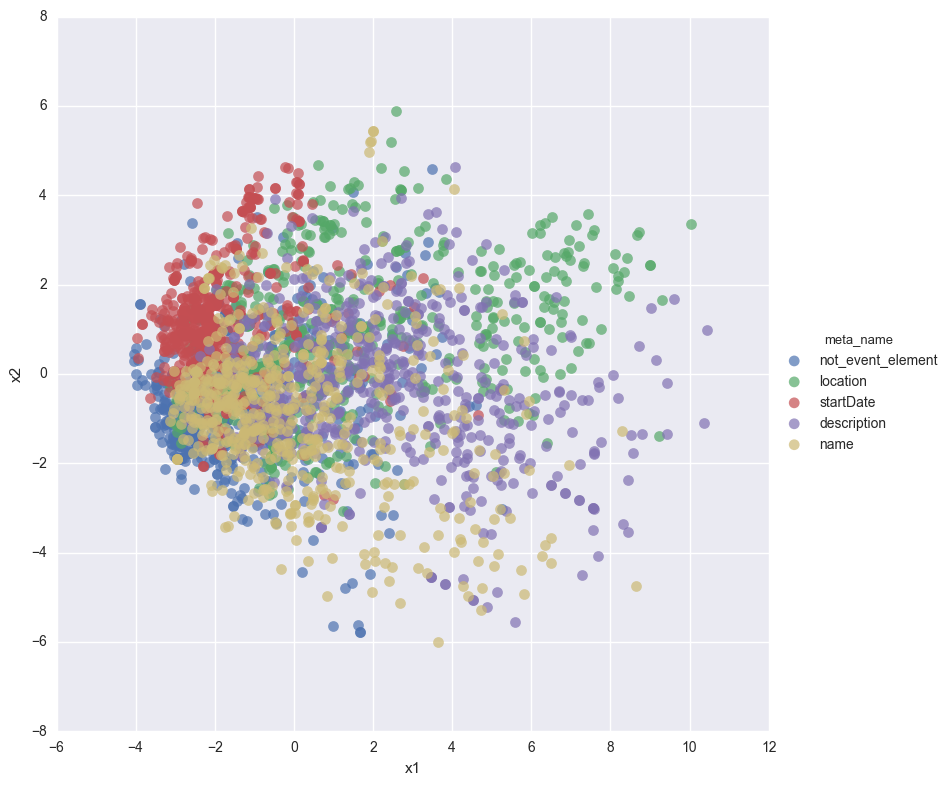
\includegraphics[width=1\textwidth]{figures07/pcatsne}
    \caption{PCA on standardized numeric values for different meta names.}
    \label{fig:pcatsne}
\end{subfigure}
% \caption{Distribution of tag and Principal component analysis}
\end{figure}

\begin{table}[h]
\begin{center}
{\renewcommand{\arraystretch}{1.5}
\begin{tabular}{| p{0.8cm} | p{2cm}|  p{2cm}|  p{2.3cm}|  p{2.3cm}|  p{2.4cm}|}
\hline
\textbf{stat}    &    \textbf{color\_r}    &    \textbf{font\_size}    &    \textbf{font\_weight}    &    \textbf{digits\_share}    &    \textbf{block\_height}\\
\hline
count    &    167872.0    &    167872.0    &    167872.0    &    167872.0    &    167872.0\\
\hline
mean    &    76.396201    &    14.69536    &    455.510746    &    0.112503    &    26.359833\\
\hline
std    &    84.989934    &    4.15742    &    129.067880    &    0.225118    &    18.612600\\
\hline
min    &    0.0    &    0.0    &    100.0    &    0.0    &    0.0\\
\hline
25\%    &    4.0    &    13.0    &    400.0    &    0.0    &    16.0\\
\hline
50\%    &    51.0    &    14.0    &    400.0    &    0.0    &    19.0\\
\hline
75\%    &    125.0    &    16.0    &    400.0    &    0.117021    &    31.0\\
\hline
max    &    255.0    &    100.0    &    900.0    &    1.0    &    194.0\\
\hline
\end{tabular}}
\caption{Summary statistics for some numerical features}
\label{table:sumstatnum}
\end{center}
\end{table} \\

\begin{comment}
Despite the fact, there are many features which visually distinguish the different meta names, dimensionality reduction output didn't show good separation. We standardized the values and performed both PCA and t-SNE approaches on all numeric features to see if the clusters appear there. Especially after unsuccessful clustering, it would be good to see it is there. PCA showed a small separation but t-SNE not. The result of PCA you can see on figure \ref{fig:pcatsne}
\end{comment}

 
\section*{Conclusion of the chapter}
In this chapter, we performed exploratory data analysis by visualizing the features and grouping by the meta names. As we see, there features which separate well the meta names (the tag, font size, digits share, text length, etc.) and which not (x and y coordinates, color). We performed dimensionality reduction with PCA and saw a small separation on clusters whereas k-means clustering on X and Y coordinates didn't perform well.  